
\chapter{\'Etudes de cas et exp\'erimentations}
\label{experiences.chap}

\gt{Pas besoin de dire que c'est <<possibilit\'es d'utilisation>>. Tu
as d\'evelopp\'e une bibloth\`eque, et tu veux voir comment elle se
compare avec d'autres.}

Ce chapitre pr\'esente une \'evaluation exp\'erimentale de \TT{PpFf} afin de comparer ses performances avec d'autres approches d'ex\'ecution parall\`ele.   

Dans les sections~\ref{wordcount.sect} et~\ref{stockprice.sect}, nous pr\'esentons deux applications de \TT{PpFf}. Ces cas d'utilisation ont \'et\'e choisis non seulement pour montrer certaines fonctionnalit\'es de l'API, mais \'egalement pour leur pertinence dans des sc\'enarios r\'eels. La section~\ref{wordcount.sect} pr\'esente une application permettant de calculer la fr\'equence d'occurrence des mots dans un texte --- le <<\emph{Hello World!} des syst\`emes de traitement de donn\'ees en mode \emph{batch} --- alors que la section~\ref{stockprice.sect} pr\'esente une application permettant de calculer des statistiques sur les prix d'indices boursiers --- un exemple typique de traitement de flux en ligne.

Mais tout d'abord, nous pr\'esentons la fa\c{c}on dont nos
exp\'erimentations ont \'et\'e effectu\'ees.

\section{M\'ethode utilis\'ee pour les exp\'erimentations}

Chaque syst\`eme informatique a des caract\'eristiques propres. Les principaux facteurs qui influencent la performance d'un tel syst\`eme sont le processeur et la communication interne. Afin d'avoir de r\'esultats pr\'ecis, nous avons conduit nos exp\'eriences sur deux machines diff\'erentes. La premi\`ere machine est une machine avec 16 processeurs avec 2,6 GHz, chacun contenant 6 cœurs. Au total, nous avons une machine à 96 cœurs fonctionnant sous Linux avec la version 3.10.0. La deuxi\`eme machine est une machine avec 64 processeurs avec 2,3 GHz, chacun contenant 8 cœurs. Le système d'op\'eration pour la derni\`ere machine est Linux avec la version 3.10.0.

Dans un environnement de traitement de flux, les donn\'ees sont g\'en\'eralement transform\'ees au fur et \`a mesure de leur progression dans le \TT{pipeline}. Chaque exp\'erience est ex\'ecut\'ee plusieurs fois pour obtenir un r\'esultat stable. Le nombre de r\'ep\'etitions de chaque exp\'erience a \'et\'e vari\'e. Dans les r\'esultats pr\'esent\'es dans les sections suivantes, nous avons pris le facteur de r\'ep\'etition pour les meilleurs r\'esultats obtenus. Donc, pour toutes les exp\'eriences ex\'ecut\'ees, le facteur de r\'ep\'etition a \'et\'e \'etabli \`a 20. Le temps d'ex\'ecution de r\'ef\'erence pour les exp\'eriences est obtenu en divisant le temps total de l'ex\'ecution au nombre de r\'ep\'etitions.


\GT{Ici, il faut donner une vue d'ensemble de la fa\c{c}on dont tu as
proc\'ed\'e~: quelles machines (architecture, OS, etc. Parler comme tu
fais ci-bas que chaque {\bf programme \emph{benchmark}} est ex\'ecut\'e
plusieurs fois, comment ce temps est mesur\'e (de l'int\'erieur du
programme par des appels syst\`emes internes), que la moyenne des
temps d'ex\'ecution est calcul\'ee pour obtenir un r\'esultat plus
juste/stable, etc.}

\GT{Ensuite, tu pourras d\'ecrire les r\'esultats pour chacun des
programmes.}

\IC{J'ai d\'ecrit un peu comment j'ai ex\'ecut\'e les tests.}



\section{Word Count}
\label{wordcount.sect}

\gt{En anglais, c'est <<appendix>> mais en fran\c{c}ais c'est annexe!}

\gt{Je crois qu'il serait pr\'ef\'erable de pr\'esenter les mesures
associ\'ees dans la m\^eme section, sinon ta section 4.2 sera courte
et ce sera m\'elangeant d'avoir les r\'esultats \`a part.}

\gt{Donc, 4.2 (idem pour 4.3) pourrait contenir: 4.2.1 Description de
l'application; 4.2.2 Mesures obtenues; 4.2.3 Analyse des r\'esultats.}

\ic{Bonne id\'ee}


\subsection{Description de l'application}

Dans la section.~\ref{descriptionWordCount.sect}, nous avons pr\'esent\'e \TT{WordCount}, une application simple qui compte le nombre d'occurrences des divers mots dans un fichier texte. L'application prend en entr\'ee un fichier texte et produit un conteneur de type \TT{map<string, int>} où la cl\'e repr\'esente un mot dans le fichier et la valeur  type \TT{int}  associ\'ee repr\'esente le nombre d'occurrences du mot dans le fichier. Les codes sources des applications \TT{WordCount} en \TT{PpFf} et~\TT{Java} sont pr\'esent\'es aux annexes~\ref{sourceCodeWordCountPpFf.ann} et~\ref{sourceCodeWordCountJava.ann} respectivement.


\subsection{Mesures obtenues}


%Plots bar examples: http://pgfplots.net/tikz/examples/tag/bar-plots/

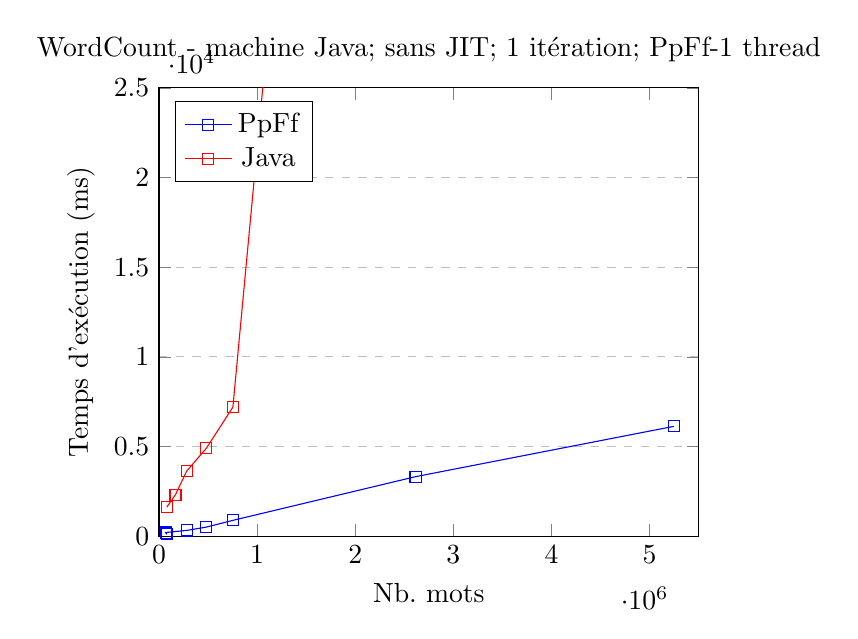
\begin{tikzpicture}
\begin{axis}[
    title={WordCount - machine Java; sans JIT; 1 itération; PpFf-1 thread\bigskip},
    xlabel={Nb.~mots},
    ylabel={Temps d'ex\'ecution (ms)},
    xmin=0, xmax=5500000,
    ymin=0, ymax=25000,
    ytick={0,5000,10000,15000,20000,25000},
    %xtick={0,500000,1000000,1500000,3000000,4500000,5000000,5500000},
    xtick={0,1000000,2000000,3000000,4000000,5000000,6000000},
    legend pos=north west,
    ymajorgrids=true,
    grid style=dashed,
]
 
\addplot[
    color=blue,
    mark=square,
    ]
    coordinates {
    (78792,106)(67941,205)(281307,322)(482636,508)(752856,883)(2614743,3320)(5247678,6126)
    };
\addplot[
    color=red,
    mark=square,
    ]
    coordinates {
    (78792,1615)(167941,2319)(281307,3625)(482636,4906)(752856,7195)(2614743,116039)(5247678,226917)
    };
\legend{PpFf,Java}    
\end{axis}
\end{tikzpicture}




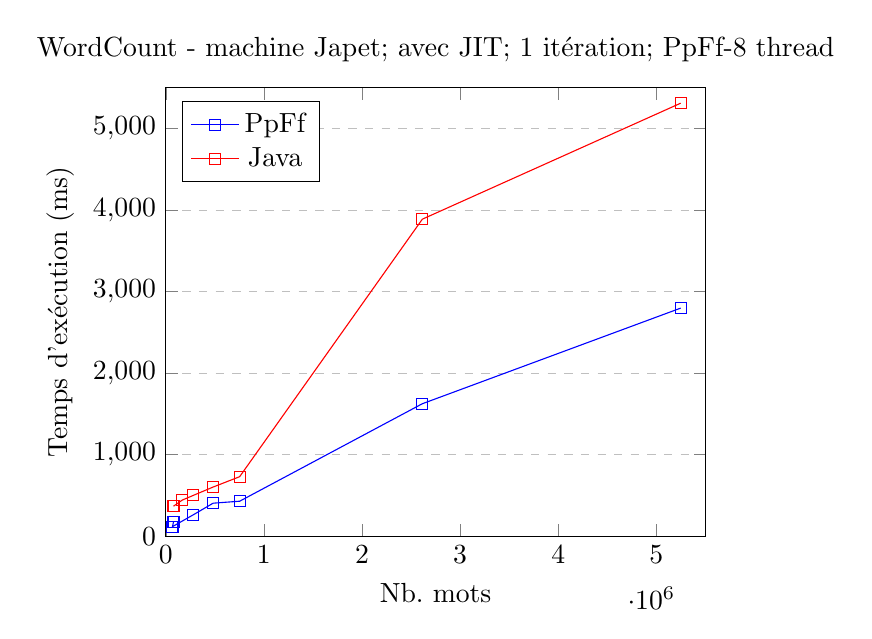
\begin{tikzpicture}
\begin{axis}[
    title={WordCount - machine Japet; avec JIT; 1 itération; PpFf-8 thread},
    xlabel={Nb.~mots},
    ylabel={Temps d'ex\'ecution (ms)},
    xmin=0, xmax=5500000,
    ymin=0, ymax=5500,
    %ytick={0,500,1000,1500,2000,2500,3000,3500,4000,4500,5000,5500},
    ytick={0,1000,2000,3000,4000,5000,6000},
    xtick={0,1000000,2000000,3000000,4000000,5000000,6000000},
    legend pos=north west,
    ymajorgrids=true,
    grid style=dashed,
]
 
\addplot[
    color=blue,
    mark=square,
    ]
    coordinates {
    (78792,174)(67941,117)(281307,263)(482636,405)(752856,429)(2614743,1625)(5247678,2798)
    };
\addplot[
    color=red,
    mark=square,
    ]
    coordinates {
    (78792,368)(167941,443)(281307,501)(482636,603)(752856,730)(2614743,3889)(5247678,5312)
    };
\legend{PpFf,Java}    
\end{axis}
\end{tikzpicture}



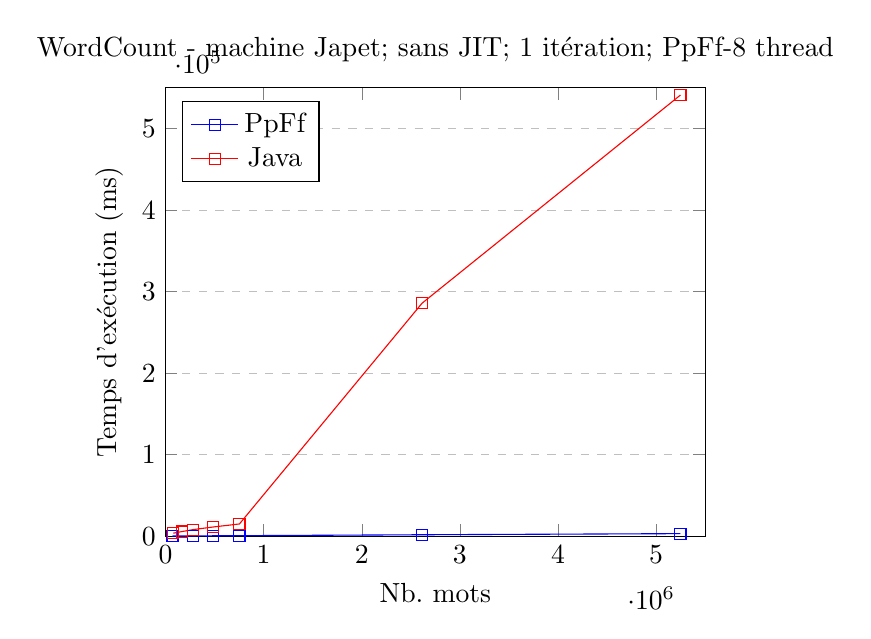
\begin{tikzpicture}
\begin{axis}[
    title={WordCount - machine Japet; sans JIT; 1 itération; PpFf-8 thread\newline},
    xlabel={Nb.~mots},
    ylabel={Temps d'ex\'ecution (ms)},
    xmin=0, xmax=5500000,
    ymin=0, ymax=550000,
    %ytick={0,100000,150000,200000,250000,300000,350000,400000,450000,500000,550000},
    ytick={0,100000,200000,300000,400000,500000,600000},
    xtick={0,1000000,2000000,3000000,4000000,5000000,6000000},
    legend pos=north west,
    ymajorgrids=true,
    grid style=dashed,
]
 
\addplot[
    color=blue,
    mark=square,
    ]
    coordinates {
    (78792,67)(67941,162)(281307,268)(482636,480)(752856,637)(2614743,1765)(5247678,3135)
    };
\addplot[
    color=red,
    mark=square,
    ]
    coordinates {
    (78792,3685)(167941,5685)(281307,8083)(482636,11258)(752856,14991)(2614743,285866)(5247678,541184)
    };
\legend{PpFf,Java}    
\end{axis}
\end{tikzpicture}




\subsection{Analyse des r\'esultats}







\section{Stock Market}
\label{stockprice.sect}

\gt{En anglais <<stock>> est, en fran\c{c}ais, une <<action (boursi\`ere)>>.}

Dans le monde informatique actuel, les institutions financi\`eres produisent d'\'enormes quantit\'es d'informations, par ex., les informations sur les march\'es boursiers. L'un des probl\`emes les plus importants qu'elles rencontrent consiste \`a trouver des moyens efficaces pour r\'esumer et visualiser les donn\'ees afin de produire des informations utiles sur le comportement du march\'e, notamment pour prendre des d\'ecisions d'investissement. Cette section pr\'esente une application qui calcule le prix maximum pour diverses actions d'un marché boursier. Les codes sources des applications \TT{StockPrice} en \TT{PpFf} et~\TT{Java} sont pr\'esent\'es dans les annexes~\ref{sourceCodeStockPricePpFf.ann} et~\ref{sourceCodeStockPriceJava.ann} respectivement. 

\subsection{Description de l'application}

L'application \TT{Stock Market} calcule le prix d'une action en utilisant le modèle \emph{Black-Scholes}~\citep{macbeth1979empirical}. Ce mod\`ele d'\'evaluation est utilis\'e pour d\'eterminer le prix juste ou la valeur th\'eorique d'une option d'achat ou de vente, et ce en fonction de six variables telles que la valeur de l'action sous-jacente, le prix d'exercice, le taux d'int\'er\^et sans risque, la volatilit\'e du prix de l'action, la dur\'ee et le type d'option. 

L'application \TT{Stock Market} est compos\'ee en un pipeline combinant cinq principales op\'erations~: 

\begin{lstlisting}[
label={exampleInfoActionFromFile},
language=c++,
caption={Un exemple illustrant l'information sur une action contenue dans un fichier.},
frame=single,
float]

SNY	100.00 90.00 0.1000 0.00 0.10 1.00 C 0.00 18.6308591206674982
\end{lstlisting}

\begin{itemize}

\item La premi\`ere op\'eration sert \`a d\'efinir la source du flux de donn\'ees. Ici, la source est constitu\'ee par les lignes contenues dans un fichier. Le listing~\ref{exampleInfoActionFromFile} montre un exemple avec quelques enregistrements tir\'es de notre fichier de test. 

Un enregistrement est identifi\'e par les informations suivantes : le nom de l'action, la valeur actuelle de l'action sous-jacente, le prix d'exercice, le taux d'int\'er\^et sans risque, le taux de dividende, la volatilit\'e du prix de l'action, le temps qu'il reste \`a l'option avant son \'ech\'eance (exprim\'e en ann\'ees), le type d'option (\TT{C=CALL}~: prix pour une option d'achat et \TT{P=PUT}~: prix pour une option de vente), la valeur de dividende et la valeur de r\'ef\'erence \TT{DerivaGem}. 
Les valeurs \TT{DerivaGem}, la valeur et le taux de dividende ne sont pas utilis\'es dans \TT{Stock Market} pour calculer le prix d'une action.

\GT{Je sugg\`ere, dans le listing, de mettre quelques
lignes/enregistrements, pas un seul --- disons une dizaine?}


\item La deuxi\`eme op\'eration permet de r\'epartir les \'el\'ements du flux entre divers \emph{threads}.
Toutes les \'etapes suivant cette op\'eration seront donc ex\'ecut\'ees en parall\`ele.

\item La troisi\`eme op\'eration,  \TT{map}, permet d'extraire le nom et les options de chaque action.

\gt{En fait, que contient un enregistrement: les infos sur une action
sp\'ecifique? Ou une transaction boursi\`ere? \`A clarifier!}

\ic{Bonne question. J'imagine qu'il s'agit d'actions enregistr\'ees \`a la suite de transaction boursi\`ere. J'ai regard\'e la description de Pico. Il n'y a pas beaucoup de d\'etails. https://github.com/alpha\-unito/pico/tree/master/examples/stock-market. (The stock\_pricing.cpp code is an example of batch pipeline (like word\-count), meaning file\-based I\/O. It takes in input a series of stock records and computes the maximum price for each stock name.) }

\item  Le prix de chaque action est calcul\'e dans la quatri\`eme op\'eration. L'algorithme utilis\'e est \emph{Black \& Scholes}~\cite{macbeth1979empirical}. 

\item Finalement, la derni\`ere op\'eration permet d'extraire le prix maximum pour chaque action.


\end{itemize}

\subsection{Mesures obtenues}


\pgfplotstableread[row sep=\\,col sep=&]{
    interval & PpFf & Java \\
    Java-JIT  & 302 & 574 \\
    Java-NO-JIT   & 504 & 2696 \\
    Japet-JIT   & 357 & 402 \\
    Japet-NO-JIT   & 350 & 5810 \\
    }\mydata

\begin{tikzpicture}
    \begin{axis}[
    		title = Temps d'ex\'ecution pour StockPrice,
            ybar,
            bar width=.5cm,
            width=.7\textwidth,
            height=.5\textwidth,
            legend style={at={(0.5,1)},
                anchor=north,legend columns=-1},
            symbolic x coords={Java-JIT, Java-NO-JIT, Japet-JIT, Japet-NO-JIT},
            xtick=data,
            nodes near coords,
            nodes near coords align={vertical},
            ymin=0,ymax=6000,
            ylabel={Temps d'ex\'ecution (ms)},
        ]
        \addplot table[x=interval,y=PpFf]{\mydata};
        \addplot table[x=interval,y=Java]{\mydata};
        \legend{PpFf, Java}
    \end{axis}
\end{tikzpicture}



\subsection{Analyse des r\'esultats}












